\documentclass[12pt,a4paper]{article}
\usepackage[catalan]{babel}
\usepackage[utf8]{inputenc}

\usepackage[right=2cm,left=3cm,top=4cm,bottom=2cm,headsep=0.5cm,footskip=0.5cm]{geometry}
\usepackage{graphicx,subfigure}
\usepackage{amsmath,amssymb}
\usepackage{underscore}
\usepackage{fancyhdr}
\usepackage{array}
\usepackage{yhmath}

\graphicspath{ {img/} }

\pagestyle{fancy}
\fancyhf{}
\rhead{\textbf{Alberto Navalón Lillo}}
\lhead{\textit{Funcions}}

\begin{document}

\section{Funcions quadràtiques}

Les funcions quadràtiques es formen partint de l'equació \(y = ax^2+bx+c\), on \(ax^2\) és el terme \textbf{quadràtic}, \(bx\) és el terme \textbf{lineal} i \(c\) el terme \textbf{independent}. Aquestes funcions tenen forma de paràbola, les quals son simètriques. El domini són tots els nombres des de \(\infty \text{ fins a } -\infty\). Per tant, aquestes funcions sempre són contínues i tenen un eix de simetria.\\

Tornant a l'equació \(y = ax^2+bx+c\), si modifiquem el valor de la variable \(a\), l'amplària de la paràbola canvia, fins al punt en que es converteix en lineal quan \(a = 0\), ja que tot el terme quadràtic s'anula, i quedaria la funció \(y = bx+c\), on no hi ha cap terme de grau 2. Si en canvi modifiquem el terme lineal \(b\), la paràbola canvia de forma què el punt més baix es desplaça per el recorregut de la paràbola inversa, es a dir, la resultant de la funció \(y = -ax^2+bx+c\). Si modifiquem el valor del terme independent, la funció simplement es desplaça verticalment.

\section{Funcions racionals}

Les funcions racionals tenen la forma \(f(x) = \frac{k}{x}\), on \(f(x)\) es veu representada de la següent manera per a \(k = 1\) (figura A):

\begin{figure}[h]
	\centering
	\subfigure[Fig. A: representació de la funció racional \textit{estàndard}.]{
		\label{fig:a}
		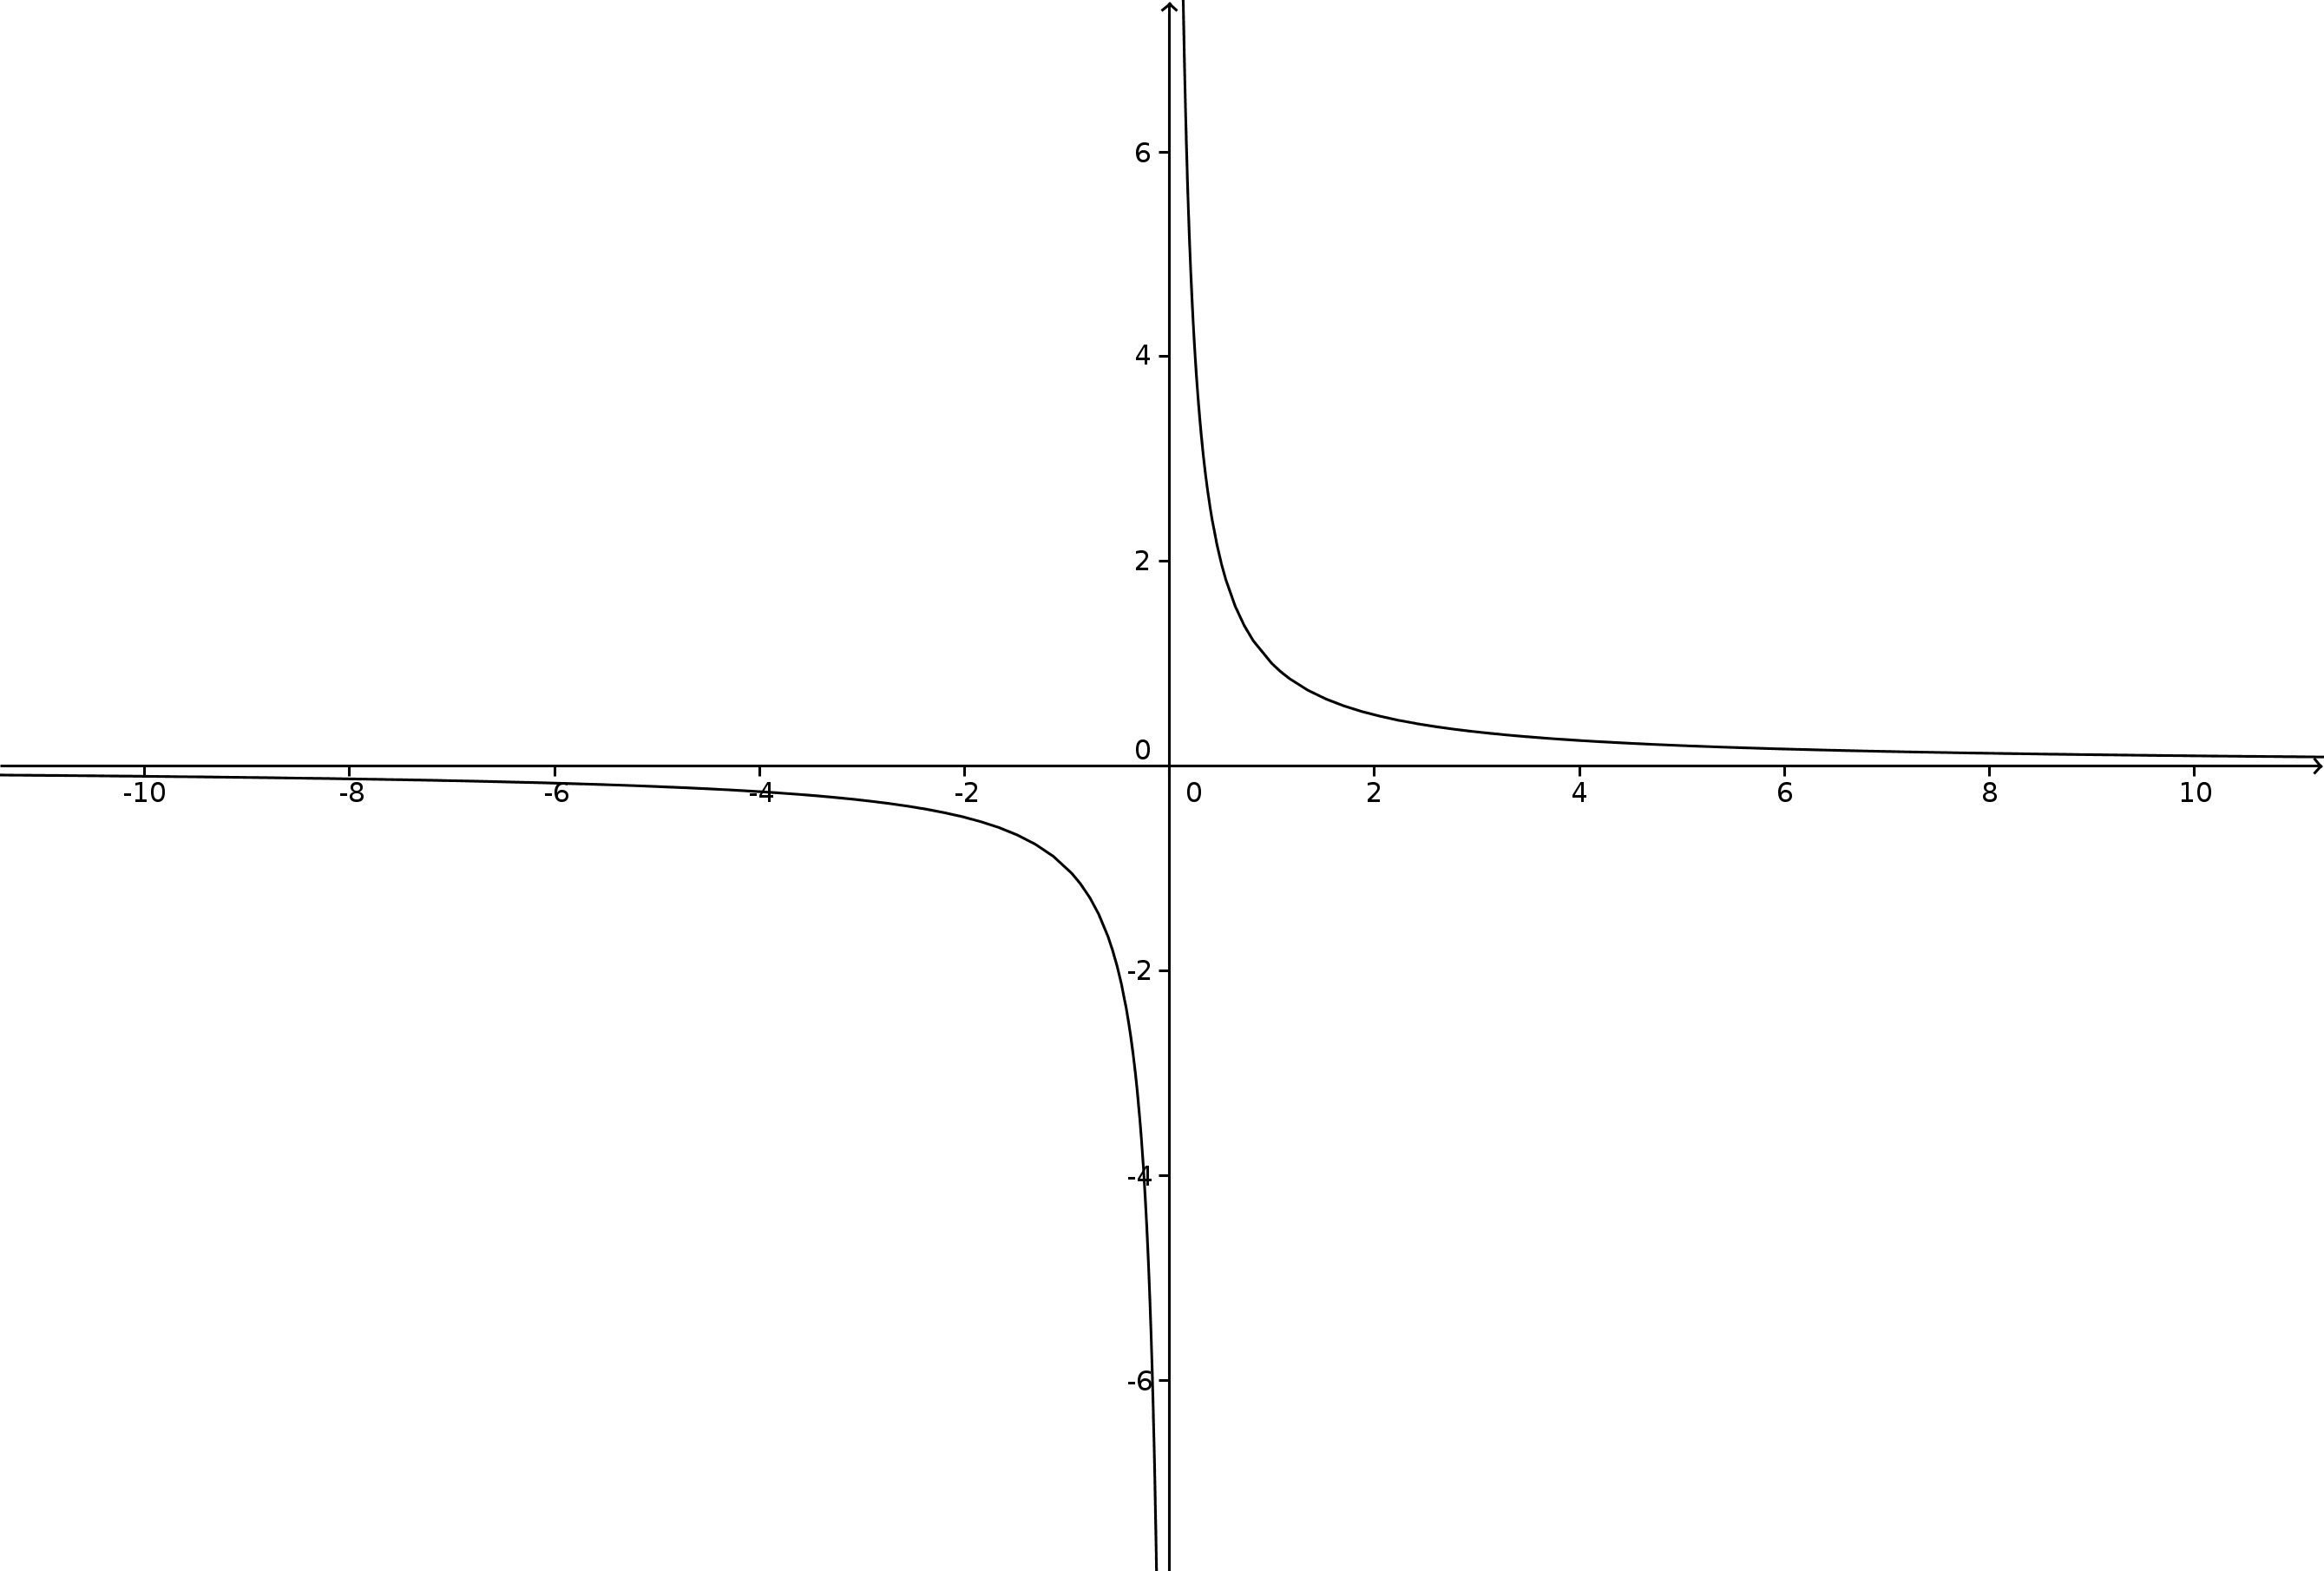
\includegraphics[width=10cm]{funcioracional}
	}
\end{figure}

De la mateixa forma, la funció inversa es pot treure amb \(g(x) = \frac{-k}{x}\). En el cas de les funcions racionals, hi existirà una asímptota sobre l'eix \(y\) en el punt en què el denominador a la funció \(f(x) = \frac{k}{x}\) siga zero, ja que la divisió entre zero és infinit. Si aproximem els límits:

\[
	f(0) \simeq \lim\limits_{x \to 0^\text{+}}\frac{k}{x} = +\infty \text{ (des del costat positiu)}
\]
\[
f(0) \simeq \lim\limits_{x \to 0^\text{-}}\frac{k}{x} = -\infty \text{ (des del costat negatiu)}
\]

També hi ha una asímptota horitzontal per un motiu similar: \(x\) sempre s'aproxima a 0.

\section{Translació de funcions exponencials}

Ja que les funcions exponencials tenen la forma \(f(x) = a^x\), la translació és una tasca molt senzilla. Per a traslladar la funció sobre l'eix \textit{x}, simplement es modifica l'exponent, de la forma \(g(x) = a^{x+n} \mid n \neq 0\). Si \(n > 0\), la funció es traslladarà cap al costat negatiu de l'eix \textit{x}. Si \(n < 0\), ho farà cap al costat positiu.\\

De la mateixa forma, podem traslladar-la sobre l'eix \textit{y}, amb una simple suma a la funció sencera, de la forma \(h(x) = a^x+m \mid m \neq 0\). Si \(m > 0\), la funció es desplaça cap al costat positiu de l'eix \textit{y}. Si, en canvi, \(m < 0\), ho farà cap al costat negatiu. Independentment d'açò, d'aquesta forma l'asímptota horitzontal es desplaçarà \(m\) unitats sobre l'eix \textit{y}.

\section{Representació gràfica de funcions trigonomètriques}

Tenim la següent funció trigonomètrica:

\[
	y = 3\cos(3x-\pi)
\]

Com que s'està fent ús de \(\pi\) i no un valor determinat de graus (90º, 180º, 270º...), hem de fer els càlculs en \textbf{radians}. En el cas d'aquestes funcions, \(\pi = 180\text{º}\), i conseqüentment, \(2\pi = 360\text{º}\). Ara podem traure una taula de valors per a \(x \text{ i } y\), la qual resulta en:

\begin{center}
	\noindent\begin{tabular}{ | >{\centering\arraybackslash}p{5cm} | >{\centering\arraybackslash}p{5cm} | }
		\hline
		\textbf{\textit{x}}	& \textbf{\textit{y}}	\\\hline
		\(\pi/3\) 			& 3						\\\hline
		\(\pi/2\)			& 0						\\\hline
		\(2\pi/3\)			& -3					\\\hline
		\(5\pi/3\)			& 0						\\\hline
		\(\pi\)				& 3						\\\hline
		0					& -3					\\\hline
	\end{tabular}
\end{center}

Partint d'aquests valors podem representar la funció, que es veu de la següent manera:

\begin{figure}[h]
	\centering
	\subfigure[Fig. B: representació gràfica de la funció \(y = 3\cos(3x-\pi)\)]{
		\label{fig:b}
		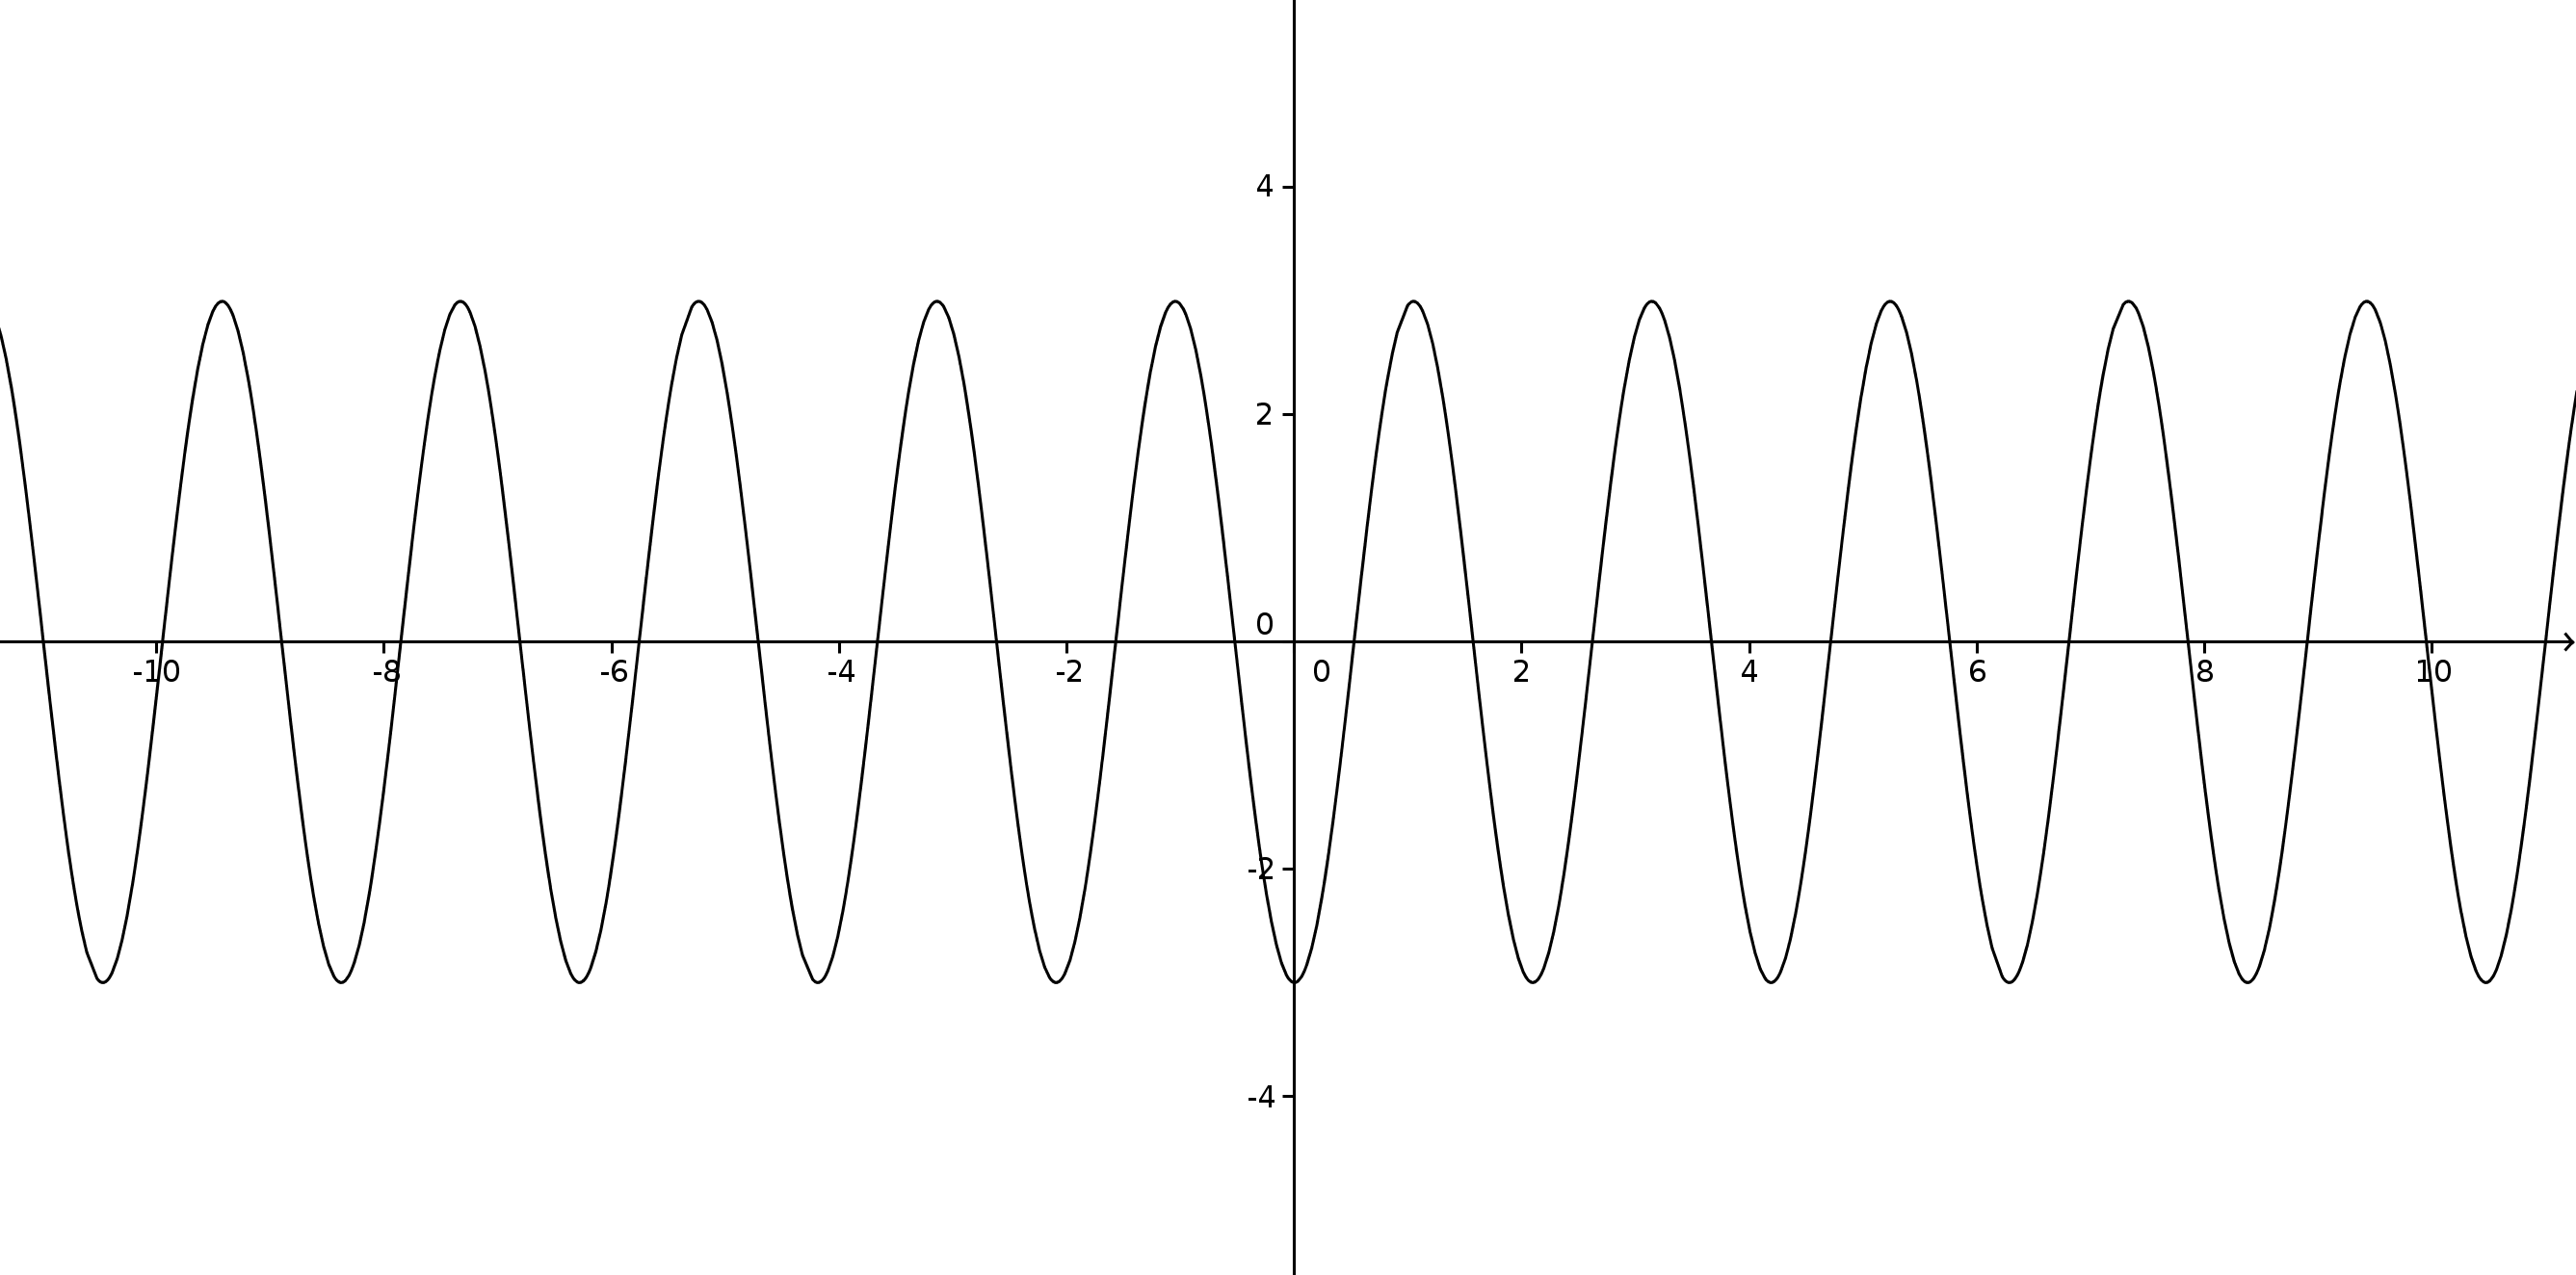
\includegraphics[width=10cm]{funciotrigonometrica}
	}
\end{figure}

\end{document}